\documentclass[12pt, leqno]{article} %% use to set typesize
\input{common}

\usepackage{fontspec}
\usepackage{polyglossia}
\setmonofont{DejaVu Sans Mono}[Scale=MatchLowercase]
\usepackage[outputdir=pdf]{minted}

\providecommand{\tightlist}{%
  \setlength{\itemsep}{0pt}\setlength{\parskip}{0pt}}
\begin{document}



\hdr{2023-04-21}

\section{Pacing the Path}

So far, we have focused on nonlinear equations
(\(f : {\mathbb{R}}^n \rightarrow {\mathbb{R}}^n\)) and optimization
problems (\(\phi : {\mathbb{R}}^n \rightarrow {\mathbb{R}}\)). Often,
though, nonlinear equations and optimization problems depend on some
extra parameter. For example:

\begin{itemize}
\tightlist
\item
  In fitting problems, we care about the solution as a function of a
  regularization parameter.
\item
  In population biology, we care about equilibrium population levels as
  a function of various parameters: birth rates, death rates, initial
  population sizes, etc.
\item
  In mechanics, we care about the deformation of a structure as a
  function of load.
\item
  In chemical kinetics, we care about equilibrium chemical
  concentrations as a function of temperature.
\item
  In engineering problems involving a tradeoff between two parameters
  (e.g.~mass and stiffness), we care about the optimal setting of one
  parameter given a fixed value of the other.
\item
  In stochastic problems, we may care about the behavior as a function
  of the variance of the noise term, or perhaps as a function of an
  autocorrelation time.
\end{itemize}

In each case, a solution path is an
\href{https://en.wikipedia.org/wiki/Implicit_function_theorem}{implicit
function} of the extra parameter. For these types of problems,
\emph{continuation} strategies are often a good choice. The basic
picture in a continuation strategy for solutions of an equation
\(F(x(s),s) = 0\) where
\(F : {\mathbb{R}}^n \times {\mathbb{R}}\rightarrow {\mathbb{R}}^n\)
starting from some easily computed solution \(x(s_0)\) is:

\begin{itemize}
\tightlist
\item
  Given \(x(s_j)\), choose a new \(s' = s_j + \Delta s\).
\item
  \emph{Predict} \(x(s')\) based on the behavior at \(s\). Two common
  predictors are

  \begin{itemize}
  \tightlist
  \item
    \emph{Trivial}: Guess \(x(s') \approx x(s_j)\).
  \item
    \emph{Euler:} Guess
    \(x(s') \approx x(s_j) - \frac{\partial F}{\partial x}(x_j,s_j)^{-1} \frac{\partial F}{\partial s}(x_j,s_j)\).
  \end{itemize}
\item
  \emph{Correct} by taking a few steps of Newton iteration.
\item
  Either \emph{accept} \(s_{j+1} = s'\) and a corresponding \(x(s_j)\)
  if the Newton iteration converged, or try again with a smaller
  \(\Delta s\). If the Newton iteration converges very quickly, we may
  increase \(\Delta s\).
\end{itemize}

Continuation is also natural if we really do care about a problem with
no free parameters, but we lack a good initial guess with which to start
an iterative method to solve the problem. In that case, a reasonable
strategy is often to \emph{introduce} a parameter \(s\) such that the
equations at \(s = 0\) are easy and the equations at \(s = 1\) are the
ones that we would like to solve. Such a constructed path in problem
space is sometimes called a \emph{homotopy}. In many cases, one can show
that solutions are continuous (though not necessarily differentiable)
functions of the homotopy parameter, so that following a homotopy path
with sufficient care can provide \emph{all} solutions even for hard
nonlinear problems. For this reason, homotopy methods are particularly
effective for solving systems of polynomial equations. Another very
popular family of homotopy methods are the interior point methods for
constrained optimization problems, which we will touch on briefly next
week.

\section{Tough to Trace}

As a starting example, let's consider a variation on the equation from
one of our first nonlinear systems lectures, a discretization of the
thermal blowup equation \[\frac{d^2 u}{dx^2} + \exp(\gamma u) = 0\]
subject to \(u(0) = u(1) = 0\). As before, we approximate the derivative
with a mesh to get a system of equations of the form
\[h^{-2} \left( u_{j-1}-2u_j+u_{j+1} \right) + \exp(\gamma u_j) = 0\]
where \(u_j\) is the approximate solution at a mesh point \(x_j = jh\)
with \(h = 1/(N+1)\). The boundary conditions are \(u_0 = u_{N+1} = 0\),
and the difference equations govern the behavior on the interior.
Compared to the last time we saw this system, though, we have introduced
a new feature: the rate constant \(\gamma\).

\begin{minted}{julia}
function autocatalytic(v, γ)
    N = length(v)
    fv        = exp.(γ*v)
    fv        -= 2*(N+1)^2*v
    fv[1:N-1] += (N+1)^2*v[2:N  ]
    fv[2:N  ] += (N+1)^2*v[1:N-1]
    fv
end
\end{minted}

\begin{minted}{julia}
function Jautocatalytic(v, γ)
    N = length(v)
    SymTridiagonal(γ*exp.(γ*v) .- 2*(N+1)^2, (N+1)^2 * ones(N-1))
end
\end{minted}

\begin{minted}{julia}
function dγ_autocatalytic(v, γ)
    v .* exp.(γ*v)
end
\end{minted}

When \(\gamma\) is equal to zero, the differential equation becomes
\[\frac{d^2 u}{dx^2} + 1 = 0,\] which has the solution (subject to
boundary conditions) \[u(x; 0) = \frac{1}{2} x(1-x).\] For larger values
of \(\gamma\), things become more interesting. Based on physical
reasoning, we expect the solutions to get more unstable (and harder) as
\(\gamma\) grows. We therefore consider a strategy in which we
incrementally increase \(\gamma\), at each point using a trivial
predictor (the solution for the previous \(\gamma\)) as an initial guess
for a Newton iteration. If the Newton iteration does not converge in a
few steps, we try again with a smaller step, stopping once the step size
has become too small.

As we get just past \(\gamma = 3.5\), the solution becomes more and more
sensitive to small changes in \(\gamma\), and we have to take shorter
steps in order to get convergence. This is reflective of an interesting
physical phenomenon known as a bifurcation. Mathematically, what we see
is the effect of the Jacobian becoming closer and closer to singular at
the solution.

\begin{figure}
\begin{center}
  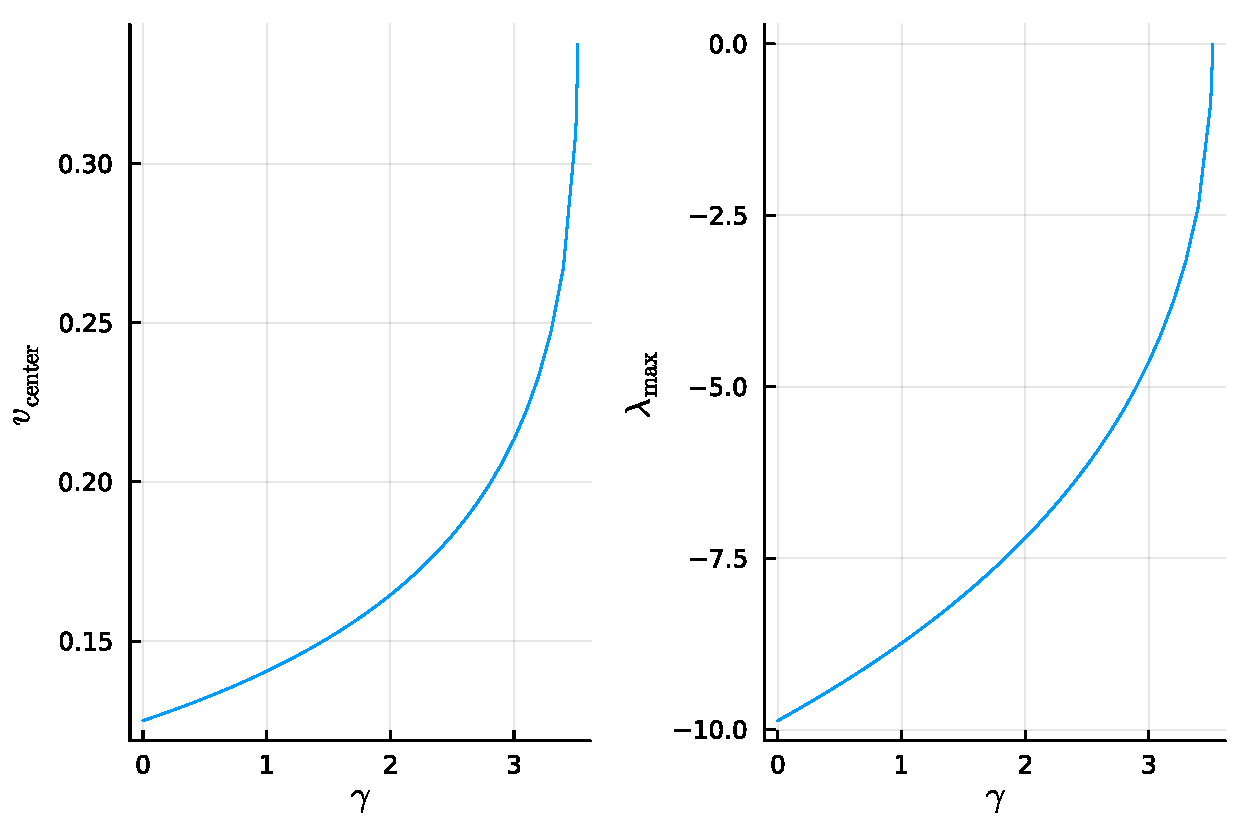
\includegraphics[width=0.8\textwidth]{fig/2023-04-21-bif0.pdf}
\end{center}
\caption{Diagram for center temperature vs $\gamma$ from 
  continuation in $\gamma$ (left) and max eigenvalue vs $\gamma$ (right).}
\label{fig:bif0}
\end{figure}

We show both the center tempertaure and the largest eigenvalue as a
function of $\gamma$ in Figure~\ref{fig:bif0}.

\begin{minted}{julia}
let
    xall = range(0.0, 1.0, length=200)
    xint = xall[2:199]
    
    # Keep a record of parameters, step sizes, and center temperatures
    γs = []
    Δγs = []
    vcenter = []
    λs = []
    
    # Current solution + storage for Newton iterates
    v = xint.*(1.0 .- xint)/2
    vnew = copy(v)
    
    γ = 0.0
    Δγ = 0.1
    while Δγ >= 1e-6 && γ < 4.0
        
	# Run Newton iteration
	converged = false
	vnew[:] = v
	for k = 1:10
	    fv = autocatalytic(vnew, γ)
	    vnew[:] -= Jautocatalytic(vnew, γ)\fv
	    if norm(fv) < 1e-8
	        converged = true
	        break
	    end
	end
    
	# Record the step if converged; otherwise, cut the
        # step size and try again
	if converged
	    v[:] = vnew
	    push!(γs, γ)
	        push!(Δγs, Δγ)
	    push!(vcenter, v[99])
	    push!(λs, maximum(eigvals(Jautocatalytic(v, γ))))
	    γ += Δγ
	else
	    γ -= Δγ
	    Δγ /= 2
	    γ += Δγ
	end
    end

    p1 = plot(γs, vcenter,
              xlabel="\$\\gamma\$", ylabel="\$v_{\\mathrm{center}}\$",
              legend=false)
    p2 = plot(γs, λs,
              xlabel="\$\\gamma\$", ylabel="\$\\lambda_{\\max}\$",
              legend=false)
    plot(p1, p2, layout=(1, 2))
end
\end{minted}

\section{Picking parameters}

In the previous section, we saw that continuation allowed us to march
\(\gamma\) right up to some critical parameter, but not beyond. We can
get a clearer picture of what is going on --- and better solver
stability --- if we look at the same problem as a function of a
\emph{different parameter} In particular, let us consider controlling
the midpoint value \(\mu\), and letting both \(v\) and \(\gamma\) be
implicit functions of the midpoint value. That is, we have the equations
\[F(v,\gamma; \mu) =
  \begin{bmatrix}
    -h^{-2} T_N v + \exp(\gamma v) \\
    e_{\mathrm{mid}}^T v - \mu
  \end{bmatrix} = 0\] with the Jacobian matrix (with respect to \(v\)
and \(\gamma\)) \[\frac{\partial F}{\partial (v,\gamma)} =
  \begin{bmatrix}
    -h^2 T_n + \gamma \operatorname{diag}(\exp(\gamma v)) &
    v \odot \exp(\gamma v) \\
    e_{\mathrm{mid}}^T & 0
  \end{bmatrix}\] where we use \(a \odot b\) to denote elementwise
multiplication. We use the same continuation process with a trivial
predictor to trace out the behavior of the midpoint as a function of
\(\gamma\).

\begin{minted}{julia}
let
    xall = range(0.0, 1.0, length=200)
    xint = xall[2:199]
    
    # Keep a record of parameters, step sizes, and center temperatures
    γs = []
    vcenter = []
    
    # Initial point
    v = xint.*(1.0 .- xint)/2
    μ = 0.125
    γ = 0.0
    
    emid = zeros(198)
    emid[99] = 1.0
    for μ in range(0.125, 2.125, length=200)
        
	# Run Newton iteration
	converged = false
	vγ = [v; γ]
	for k = 1:10
	    fvγ = [autocatalytic(vγ[1:end-1], vγ[end]); vγ[99]-μ]
            J11 = Jautocatalytic(vγ[1:end-1], vγ[end])
            dγf = dγ_autocatalytic(vγ[1:end-1], vγ[end])
	    Jvγ = [J11   dγf;
	           emid' 0.0]
	    vγ[:] -= Jvγ\fvγ
	    if norm(fvγ) < 1e-8
	        converged = true
	        break
	    end
	end
        
	# Record
	if converged
	    v[:] = vγ[1:end-1]
	    γ = vγ[end]
	    push!(γs, γ)
	    push!(vcenter, v[99])
	else
	    println("Nonconvergence at $μ = μ")
	    break
	end
        
    end
    
    # Say where we stopped and plot some diagnostics
    plot(γs, vcenter, xlabel="\$\\gamma\$", ylabel="\$v_{\\mathrm{center}}\$",
         legend=false)
end
\end{minted}

\begin{figure}
\begin{center}
  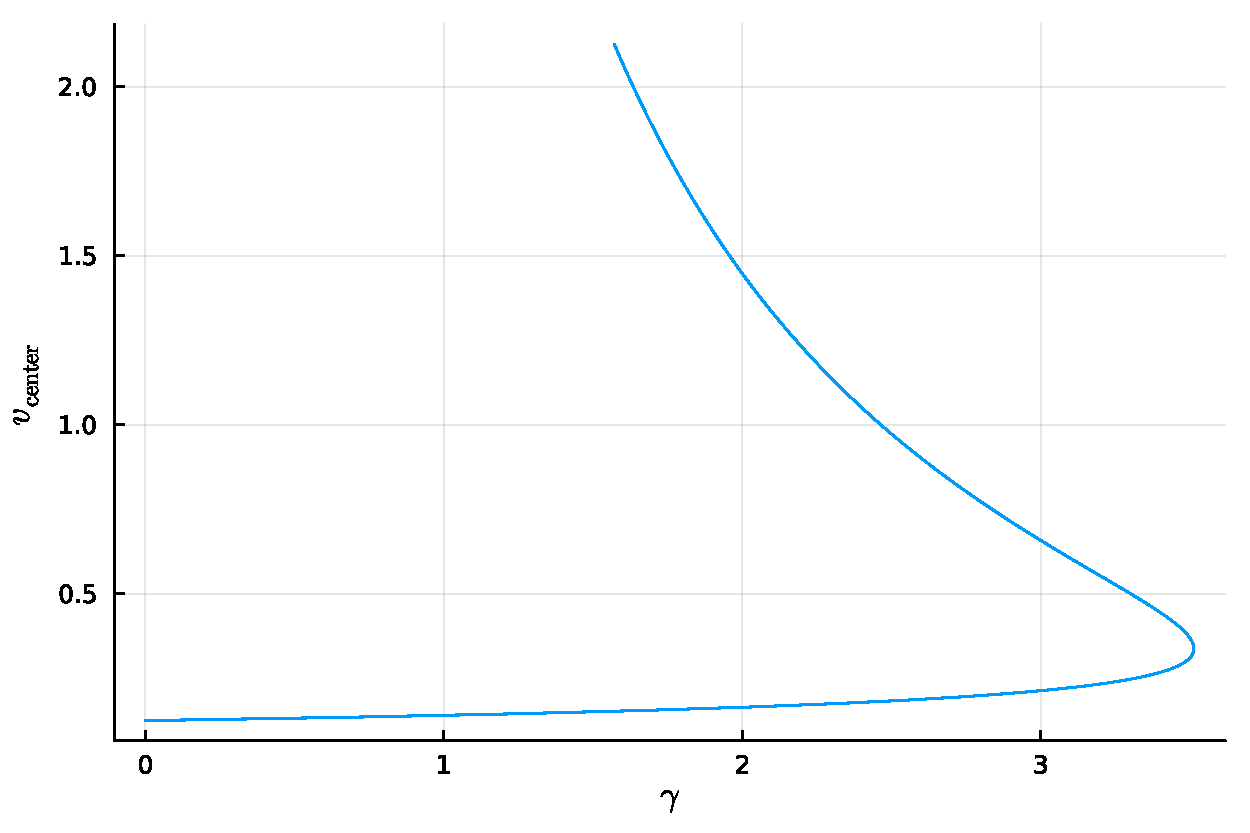
\includegraphics[width=0.8\textwidth]{fig/2023-04-21-bif1.pdf}
\end{center}
\caption{Diagram for center temperature vs $\gamma$ from continuation in
  center temperature.}
\label{fig:bif1}
\end{figure}

The result of this code is shown in Figure~\ref{fig:bif1}.
This picture makes the behavior of the solution close to 
$\gamma = 3.5$ a little more clear. The phenomenon shown is called a {\em fold
bifurcation}. Physically, we have that for $\gamma \lesssim 3.5$,
there are two distinct solutions (one stable and one unstable); as
$\gamma$ increases, these two solutions approach each other until at
some critical $\gamma$ value they ``meet.'' Beyond the critical value,
there is no solution to the equations.

\section{Pseudoarclength Ideas}

What if we think we might run into a fold bifurcation, but do not know a
good alternate parameter for continuation? A natural idea is to
parameterize the solution curve (e.g.~\((v(\gamma),\gamma)\)) in terms
of an \emph{arclength} parameter. In practice, we do not care too much
about exactly controlling arclength; it is just a mechanism to avoid
picking parameters. Therefore, we pursue \emph{pseudo-arclength}
strategies as an alternative.

For the simplest pseudo-arclength continuation strategy, consider a
function \(F : {\mathbb{R}}^{n+1} \rightarrow {\mathbb{R}}^n\). Assuming
the Jacobian has maximal rank, we expect there to be a solution curve
\(x : {\mathbb{R}}\rightarrow {\mathbb{R}}^n\) such that
\(F(x(s)) = 0\). The null vector of the Jacobian \(F'\) is tangent to
\(x\), and so we can use this to predict a new point. The basic
procedure to get a new point on the curve starting from \(x^j\) is then:

\begin{itemize}
\tightlist
\item
  Consider the Jacobian \(F'(x^j) \in {\mathbb{R}}^{n \times (n+1)}\)
  and compute a null vector \(v\) (a simple approach is to compute a QR
  factorization). Choose a tangent vector \(t^j \propto v\); usually we
  normalize so that \(t^{j-1} \cdot t^j > 0\).
\item
  Move a short distance along the tangent direction (Euler predictor),
  or otherwise predict a new point.
\item
  Correct back to the curve. One approach is the iteration
  \[y^{k+1} = y^k - F'(y^k)^\dagger F(y^k)\] where
  \(F'(y^k)^\dagger \in {\mathbb{R}}^{(n+1) \times n}\) is the
  pseudoinverse of the Jacobian. This is equivalent to solving the
  problem
  \[\mbox{minimize } \|p^k\|^2 \mbox{ s.t. } F'(y^k) p^k = -F(y^k).\]
\item
  If the iteration curves and the new point is OK, accept the point and
  move on. Otherwise, reject the point and try again with a shorter step
  in the tangent direction.
\end{itemize}

Depending on what linear algebra tools are available to you, you may
choose different strategies to compute the tangent vector or correct
back to the curve. Indeed, some peculiarities in the Julia sparse
rectangular solvers leads us to prefer something different.

\begin{minted}{julia}
let
    xall = range(0.0, 1.0, length=200)
    xint = xall[2:199]

    # Keep a record of parameters, step sizes, and center temperatures
    γs = []
    vcenter = []
    
    # Initial point
    v = xint.*(1.0 .- xint)/2
    γ = 0.0
    μ = 0.125
    
    # Indicator for last column (used for tangent vec)
    eγ = zeros(199)
    eγ[end] = 1

    # Take an initial vector to establish direction to move on curve
    tprev = zeros(199)
    tprev[99] = 1
    
    while v[99] <= 2.0
        
	# Compute a tangent vector in the same direction as before
	J = [Jautocatalytic(v, γ)  dγ_autocatalytic(v, γ) ; tprev' ]
	t = J\eγ
	t /= norm(t)
	tprev[:] = t
        
	# Take Euler predictor step
	h = 0.1
	vγ = [v; γ] + h*t
        
	# Correct back to curve
	converged = false
	for k = 1:10
	    fvγ = autocatalytic(vγ[1:end-1], vγ[end])
	    J11 = Jautocatalytic(vγ[1:end-1], vγ[end])
            dγf = dγ_autocatalytic(vγ[1:end-1], vγ[end])
            Jvγ = [J11 dγf; t']
    	    vγ[:] -= Jvγ\[fvγ; 0]
	    if norm(fvγ) < 1e-8
	        converged = true
	        break
	    end
	end
        
	# Record
	if converged
	    v[:] = vγ[1:end-1]
	    γ = vγ[end]
	    push!(γs, γ)
	    push!(vcenter, v[99])
	else
	    println("Nonconvergence in corrector")
	    break
	end
        
    end
    
    plot(γs, vcenter, xlabel="\$\\gamma\$", ylabel="\$v_{\\mathrm{center}}\$",
         legend=false)
end
\end{minted}

\begin{figure}
\begin{center}
  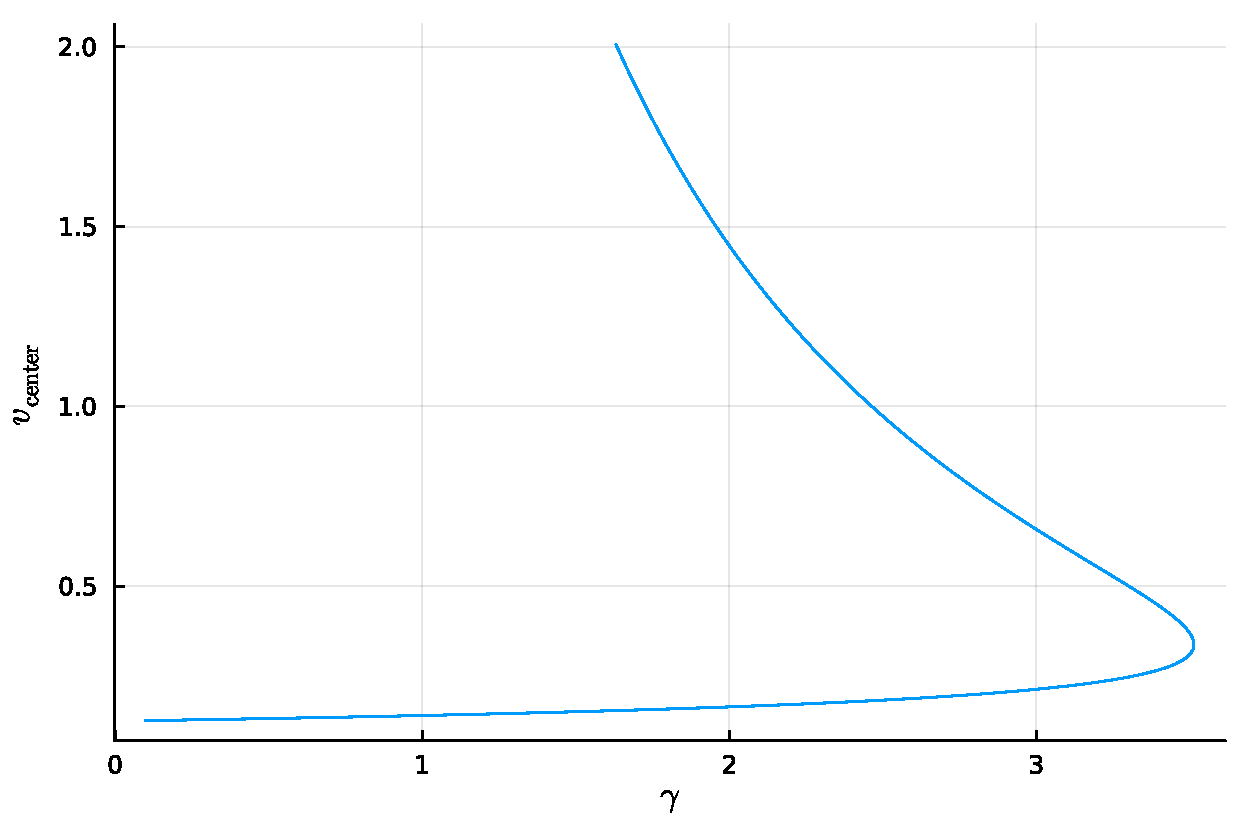
\includegraphics[width=0.8\textwidth]{fig/2023-04-21-bif2.pdf}
\end{center}
\caption{Diagram for center temperature vs $\gamma$ from pseudo-arclength
  continuation.}
\label{fig:bif2}
\end{figure}

The result of this code is shown in Figure~\ref{fig:bif2}.

\section{And Points Beyond}

There is a large and fascinating literature on numerical continuation
methods and on the numerical analysis of implicitly defined functions.
Beyond the predictor-corrector methods that we have described, there are
various other methods that address similar problems: piecewise linear
(simplex) continuation, pseudo-transient continuation, and so forth. We
can combine continuation ideas with all the other ideas that we have
described in the course; for example, one can do clever things with
Broyden updates as one walks along the curve. We can also apply step
control techniques that some of you may have learned in a class like CS
4210 in the context of methods for solving ordinary differential
equations.

A little knowledge of continuation methods can take you a long way, but
if you would like to know more, I recommend
\href{https://doi.org/10.1137/1.9780898719154}{\emph{Introduction to
Numerical Continuation Methods}} by Allgower and Georg.


\end{document}
